\documentclass{article}

\usepackage{epcc}
\usepackage{graphics}
\usepackage{booktabs}
\usepackage[colorlinks,linkcolor=black, anchorcolor=black, citecolor=black]{hyperref}
\usepackage{subfigure}

\renewcommand{\labelenumii}{\theenumii}
\renewcommand{\theenumii}{\theenumi.\arabic{enumii}.}

\begin{document}

\pagenumbering{roman}

\title{Extended Parallel I/O Benchmarks}
\author{Jiyao Lyu}
\date{\today}

\makeEPCCtitle

\newpage

\tableofcontents

\newpage
\pagenumbering{arabic}

\section{Introduction}

This project aims to extend the benchmark of parallel I/O system based on previous work, which includes Parallel IO Benchmarking \cite{ref:Wu}, benchio \cite{ref:benchio}, and Parallel I/O Performance Benchmarking and Investigation on Multiple HPC Architectures \cite{ref:archer}.

I/O performance has already become a bottleneck in High-Performance Computing (HPC) system. The reasons that serial IO is hard are as follows:

\begin{enumerate}
	\item \textbf{Breaks out of the excellent process/memory model}
	When we write a program, we have some processes that are running some data. The data in our program can be objects, arrays, or complicated data structures. When writing data to disks, the data has to go through the memory and then physically appears on the disks. Operations happen on disks are much slower than in CPU. Because hard disks are several orders of magnitude slower than the CPUs, and even much slower than the memory.

	If the order of bytes in memory is the same as in the file, then it is not complicated. There is often a re-mapping from the data structure in the program so we can write to disks, which can make things more complicated.
	\item \textbf{Different formats}
	We could have text, binary formats. We could have this problem: the data may not be portable because one compute may store a 4-byte floating number in one specific order, while another compute may store it in another order. Then we cannot be able to read it.
	\item \textbf{File systems are very complicated}
	Different operating systems have different ways of managing files (the properties and permissions set on the files are not the same).
	
    One of the most important features of Linux is its support for multiple file systems, which makes it more flexible and can coexist with many other operating systems.
    There are multiple layers of storage in modern file systems between the memory and the physical disk. E.g., Data may be cached in memory in the operating system or in memory in the disk controller. Understanding the performance is, therefore, very difficult.
\end{enumerate}

The main difference between serial and parallel IO is that, in parallel, we
have multiple processes doing IO at the same time. However, parallel IO is even harder:

\begin{enumerate}
	\item \textbf{Cannot have multiple processes writing a single file}
	Unix and Linux generally cope with this, the idea in Unix is: when we open a file, we are the only user. If we want to do parallel by MPI-IO, we are going to have lots of MPI processes reading and writing to the same file.
	
	However, this will cause another problem. When we try to use multiple processes to write a file at the same time, it will cause synchronization problems. If we cannot determine the execution order of processes, it will produce incorrect results, even cause the deadlock.
	\item \textbf{Even reading can be difficult}
	We are sure that multiple processes can open the same file but the file system was not designed to have thousands of processes to open a single file. 
	
	For Lustre File System. Although there are many disks (OSTs), there is only one MetaData Server (MDS). Opening or closing a file is done by the MDS. If we have thousands of processes opening the same file, then the MDS can become overloaded and everything slows down.
	\item \textbf{Data is distributed across different processes}
	The problem is because the data is distributed, lots of processes own lots of data of the file, we need to bring it together. In general own contiguous chunks of the file. When we want to do a 2D-decomposition with a large file, each process is going to read and write lots of different parts of the file at the same time. That can be quite difficult. We may also have junk data (e.g., halos in MPP coursework).
\end{enumerate}

For these reasons above, I plan to create a benchmark program using MPI-IO and Lustre file system with a 2D dataset in this project. Because we need a benchmark to help us measure the IO performance in different environments using different process decomposition methods (e.g., regular pattern and irregular pattern).
It can allow us to measure the highest actual operating performance of the hardware of the machine and the performance improvement effect of software optimization so that the measured computer performance can compare with the performance of other computers running the same program.
A user can easily experiment with the best approach before implementing it in full application code.
The best approach could be very different, even on two similar HPC systems.
The test results of the benchmark program directly reflect the speed at which various parts of the computer system complete various tasks, thereby making a targeted evaluation of the system. Here we should only care about the IO performance.

\section{Previous Dissertation Review}
\subsection{Summary}
Jiaying’s project used MPI-IO, NetCDF and Lustre File System operating on a 2D regular dataset. Her code was written in Fortran.

There are nine chapters in her dissertation. For the introduction part, she explained the factors that affect the efficiency of parallel, including CPU, memory, network bandwidth, IO, etc. Then she emphasized that IO is the most crucial factor because it has now become a bottleneck for HPC. Since Jiaying’s project is also based on previous work, in Chapter 2, she introduced the technology, platform, and some terms used in the literature she references, which include

\begin{enumerate}
	\item {MPI-IO and some related functions}
	\item {NetCDF and some related functions}
\end{enumerate}

Then she compares the preferences and usage of the two. It concludes that if users are more inclined to obtain higher performance, they should use MPI-IO, if they are more inclined to share data with others, NetCDF will be a better choice.
Jiaying then introduced the concepts of the parallel file system. She used Lustre File System and file striping. Figures were used to describe essential components of the file system, including Metadata Server, Object Storage Targets, etc.
Figure 1 below illustrates the implementation principle of file striping on Lustre.

Next, the author begins to explain the order of array elements in memory in the Fortran language environment and three methods of process decomposition.
We can divide the 2D-decomposition method into three types, 1x4, 4x1, and 2x2. Then the author introduces block distribution and block-cyclic distribution, as shown in Figure 2.

\begin{figure}[h]
\centering
\begin{minipage}[t]{0.8\textwidth}
\centering
\resizebox{1.00\hsize}{!}{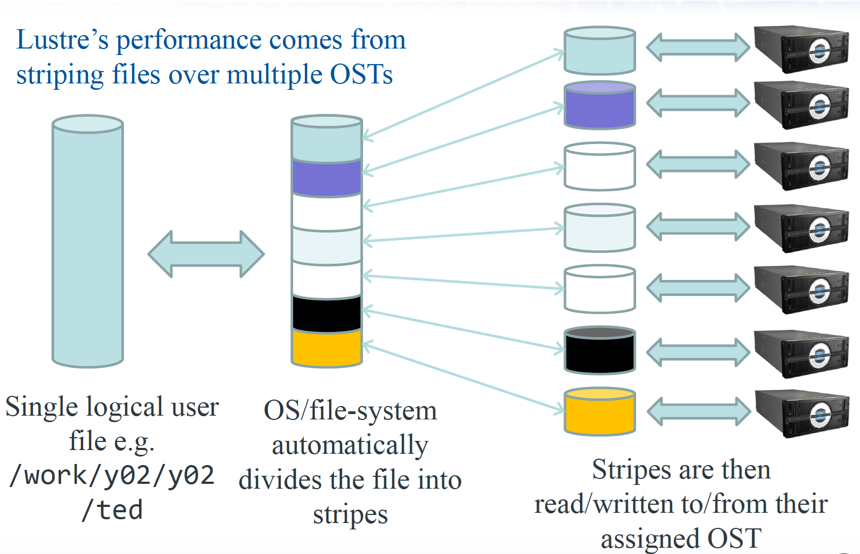
\includegraphics{logos/Lustre.png}}
\caption{Regular decomposition; extracted from the benchmark paper[1]}
\end{minipage}
\begin{minipage}[t]{0.8\textwidth}
\centering
\resizebox{1.00\hsize}{!}{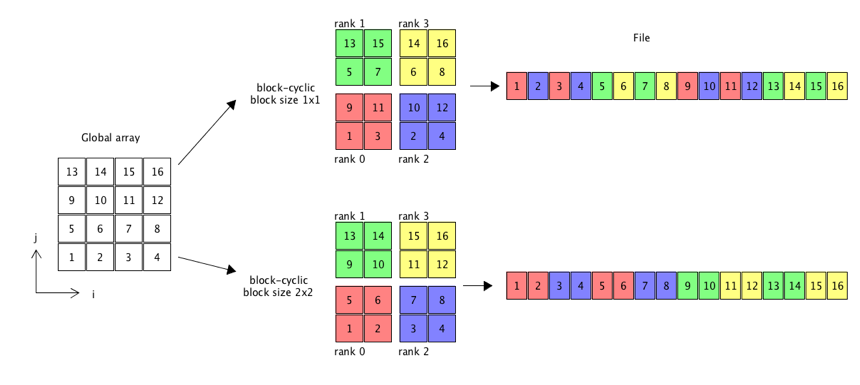
\includegraphics{logos/block-cyclic.png}}
\caption{Irregular decomposition}
\end{minipage}
\end{figure}

In Chapter 3, the author talked about experimental design. First, she introduced the hardware and software (ARCHER, Lustre File System) that will use. The entire code of her project only runs on ARCHER. Her code is an extension of the coursework from the previous Message Passing Programming (MPP) course, which is an image recovery application.
The input data in the project is a 16384x20480 single-precision floating-point array, and input files of different formats should be used for MPI and NetCDF, respectively. If we use the same decomposition approach for distribution in both the reading and writing stages, the output file of the benchmark will be identical with the input file.

The entire code execution process is roughly divided into nine steps: MPI\_Init, Read command arguments, Determine data decomposition, MPI\_Cart\_create, Determine IO pattern and data distribution, Read file, Write file, Output IO times and rates, MPI\_Finalize. Next, the author introduces these steps in detail.

In Chapters 4 to 8, she mainly explained the effects of different factors on the experimental results, including Process Counts, Process Decomposition with Block and Block-cyclic Distribution, IO Libraries, and File Striping. All factors were tested in multiple sets of tests.

Finally, the authors concluded that ARCHER could achieve IO performance improvement when we use Lustre File System, MPI-IO or NetCDF

In order to achieve higher performance, there are several recommendations:

\begin{enumerate}
	\item {IO should be a collective manner}
	\item {Minimize calls to IO read or write functions}
	\item {Lustre File System must use parallel IO for disks}
\end{enumerate}

\subsection{Evaluation}
Judging from the results, her benchmark program on ARCHER does improve IO performance. For example, MPI-IO can improve read and write rate by at least 6.5 times and 12 times in striped mode. She used the method of comparative experiments and controlling variables to get accurate results and compared the impact of different factors on IO performance.

Her experiments ran on ARCHER, which supports the Lustre File System. After loading the necessary libraries for compilation, we can run it without bugs or errors. Then obtain results successfully.

This project uses a 2d data set, and the process is assigned data using a regular composition. This article also introduces various methods of composition and distribution, such as 1x4, 2x2, block and block-cyclic, etc. However, decomposition methods described in this article are regular, which means the positions of the data responsible for each process in memory are fixed.

The writing style of the article is smooth, the logic and organization are clear, the expression is easy to understand and there are no obvious grammatical mistakes. It has a neat layout, reasonable location and size of pictures and tables. The point of view in reference has been reasonably explained; use in-text citation many times. All quoted figures and tables are correctly cited.

There are also some disadvantages. The first is she has not shown that it is portable. She decided to run it on only one machine.
To check if the program is portable, I re-compile it and re-run it on cirrus. It works normally, although, at the current stage, I can only run it on the front-end of Cirrus.
Because of the upgrade, we do not know when ARCHER2 can use. Thus, we need a program that is portable or made multiple versions to adapt to different environments. I would like to run my program on more machines.

Next, the decomposition methods in this project are all regular, which is a simple case. One significant point in my project is to extend it to an irregular pattern and then investigate the IO performance.
The irregular pattern will be explained in Section 5.

\section{Background and Literature Review}
\subsection{Summary}

For this part, I chose one paper named Performance of Parallel IO on ARCHER\cite{ref:benchio}. This paper mainly discussed I/O performance improvement on ARCHER, it used MPI-IO, and Lustre file system with a 3-dimensional dataset. IO is a bottleneck of HPC system all the time because input and output operations will take up a lot of resources, especially writing.
However, parallel IO is even harder. Master IO is not enough to get high performance and also not easy to scale.
Master IO uses only one process to read and write. In the beginning, the master process generates sub-processes to read and process data, then all the sub-process send data to the master process, and the main process writes to files.
The motivation is to explore how much performance can be improved by parallel IO. They created a benchmark program that only runs on ARCHER to achieve this.
The problem is that if we want to create an identical file in parallel as the serial one, data rearrangement is always needed because we cannot get a continuous data stream from different processes.
The solution is that processes communicate with each other on the IO stage. This paper introduced four strategies for writing data only as writing is much more difficult that reading and HPC system will also do more work on writing.

\begin{enumerate}
	\item \textbf{Multiple files, multiple writers}
	This is the simplest way and does not need data rearrangement because each process will write to a different file. However, programs that will use these data need to access multiple files.
	\item \textbf{Single file, single writer}
	This method just use one process to write. Therefore, it is also called the master IO.
	\item \textbf{Single file, multiple writers}
	This method uses multiple processes to write. However, processes will not transfer data with each other. They will write their data to the correct position. Tasks only communicate to avoid writing clashes.
	\item \textbf{Single file, collective writers}
	For this method, they created a subset of tasks for the IO stage. This subset is responsible for rearranging data and avoid clashes.
\end{enumerate}

\subsection{File system}
Next, this paper introduced the Lustre file system. It uses a technique named \textit{file striping}, which means one file separately stored on multiple disks.

Lustre file system has four basic components: Object Storage Targets, Object Storage Servers, Metadata Server and Lustre Clients. One OSS is responsible for 4 OSTs on ARCHER. Here we only concentrate on MDS and OST. Then this paper  introduced  potential issues for the four writing strategies discussed above.
To conclude, "Single file, collective writer" is the best strategy  as the IO system can guarantee no clashes happen and has the potential to reach high bandwidth and scale.

In MPI-IO library, they used routine \textit {MPI\_File\_write\_all()} to write data, which is a collective 
routine and has many benefits such as it can create a subset of tasks writers and gather data together, furthermore, it can also guarantee no clashes happen.

\subsection{Experiments}
The authors did experiments with a comparison between serial and parallel. Each of them was also divided into three parts: \textit{striped}, \textit{defstriped} \textit{unstriped}. Serial IO represents a \textit{single file, single writer} mode. Parallel IO represents \textit{single file, multiple writers} and \textit{single file, collective writers} mode.

Figure 3 shows that under weak scaling condition, serial IO performance is independent of striping methods. They are all around 500MiB/s. This result is nearly the same as unstriped parallel IO. There is another point we need to concern: we need both IO and file system are in parallel mode, or we cannot obtain the best performance.
However, for \textit{defstriped striping} mode, the results show a little difference, its peak bandwidth reached 2GiB/s because we set default defstripe striping value of 4. As for \textit{striped parallel} mode, the  highest bandwidth is proportional to the number of processes. When the number of processes is 4096, it comes to 14GiB/s.

\begin{figure}[h]
\begin{center}
\resizebox{0.80\hsize}{!}{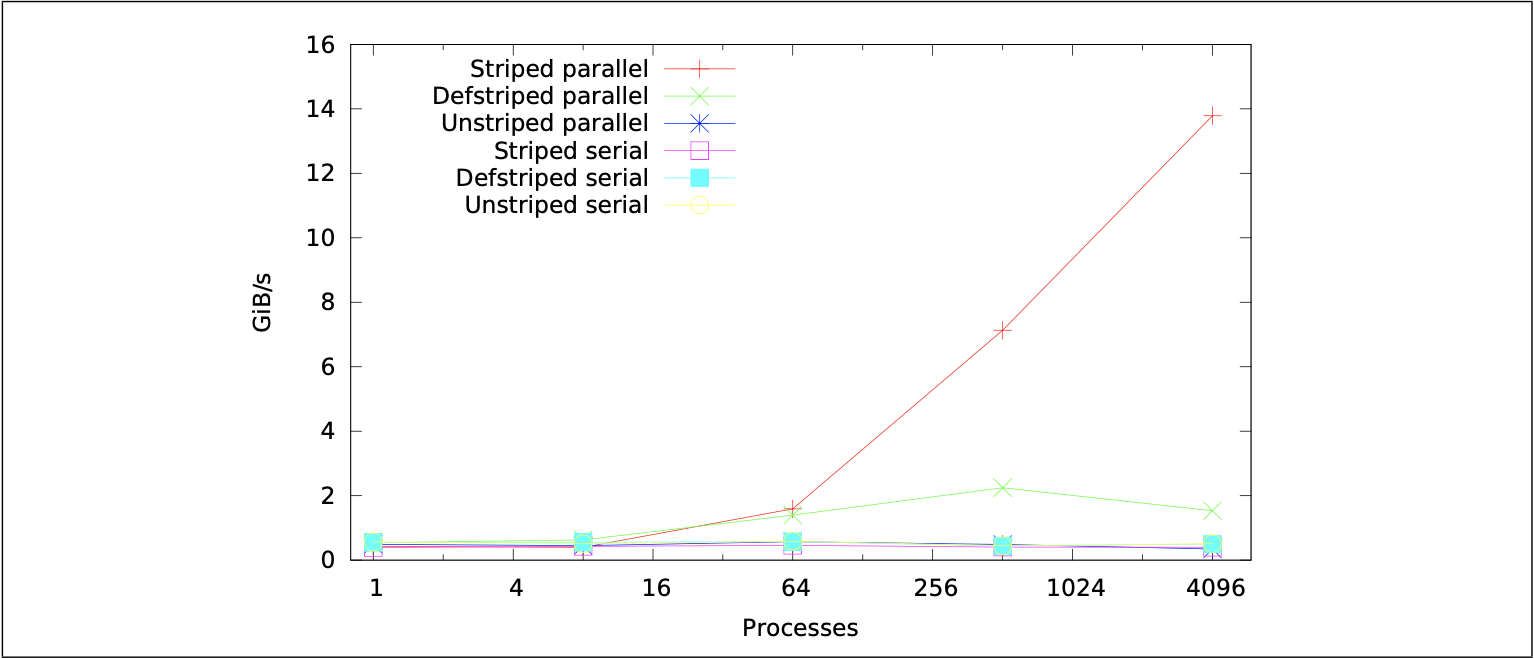
\includegraphics{logos/Figure1.png}}
\end{center}
\caption{Write bandwidth for local data volume n = 128}
\label{fig:eucrest}
\end{figure}

\subsection{Conclusion}
This paper proved that parallel IO could significantly improve performance on ARCHER. When we run the serial code, it has no difference in how we set the striping method. For \textit{defstriped striping}, the highest bandwidth will be limited by the default striping value we set. When it comes to full striped mode, the performance will increase with the number of processes. According to the theoretical analysis and results of the experiments, \textit{signle file, collective manner} is the best way for parallel IO.
In order to achieve this goal. There are three conditions must be guaranteed to get high performance.

\begin{enumerate}
	\item Parallel IO
	\item In a collective manner
	\item File must be striped
\end{enumerate}

\subsection{Assessment}
\subsubsection{Positive aspects}
This paper aims to investigate parallel IO performance improvement on ARCHER. The experiments in this article are comprehensive and rigorous. They use controlled variable method and comparative experiments then obtain conclusions that parallel IO with file striping can indeed improve performance.
The format is very structured, figures and tables are easy to understand.

\subsubsection{Negative aspects}
We may need more data comparisons to support the conclusions. For example, we can not only assume that data size \textit{n} is equal to 128 and 256 but also has more values.
This paper also did not give what data format they used, such as HDF5, NetCDF.
We could explore some other parallel IO libraries other than MPI-IO and try other parallel file systems, probably on some different machines. Then we can compare its performance in more aspects.

Another point is that this paper only looks at simple, regular decompositions. This is a motivation for my work to compare the results with irregular decompositions.

\section{Preliminary Investigations}
\subsection{Re-run Jiaying's code}
Re-run Jiaying's code is very important. The results of running her code can give us a reference for performance. One of my tasks in this project is to rewrite this program in C. The results of her code will help to check whether the C program is correct and can get the same performance.
Jiaying's coding part of her project is Fortran version. While the code was only run on ARCHER. However, since ARCHER may be out of service recently, that time, we cannot use it anymore. Therefore, we should find another machine that can run the code stably. Cirrus and ARCHER 2 are considered, while we still have no idea when ARCHER 2 will be available. Finally, I ran her code on Cirrus instead.
After uploading the code to Cirrus, we need to load two modules to enable us to compile. One is \textit{mpt}; the other is \textit{intel-compilers-18}. This time we do not need to load the modules that have been loaded on ARCHER because Cirrus does not provide them.
Then we also need to make some changes to \textit{Makefile} because there is some difference between these two machines exists. "-fastsse" flag in line 18 should be deleted because it is not a suitable flag on Cirrus.

\subsection{Results of Jiaying's code}
After compiling, we still need to create an input file for the program because the original version does not provide it. David has created a file named \textit{mkfile.f90}. It can generate input data, which are 2-dimensional datasets. Afterward, her code can run on the front-end of Cirrus using command \textit{mpirun -n 4 ./benchmark 1 1 input2048x1024.dat defstriped 2 2 1 1} and produce some screen output successfully.

Here are some results from Cirrus:

\begin{verbatim}
Hello from rank            0 , processor name is indy2-login0
Hello from rank            1 , processor name is indy2-login0
Hello from rank            2 , processor name is indy2-login0
Hello from rank            3 , processor name is indy2-login0

iInIOLib=           1 iOutIOLib=           1
filename=input2048x1024.dat striping=defstriped
aiDims=           2           2
iInDistribType=           1  distribs(iInDistribType)=SUBARRAY
iOutDistribType=           1  distribs(iOutDistribType)=SUBARRAY
aiBlockSizes=          16          16

Numbers of processes in each dimension            2 ,            2
Processing         2048  x         1024  image

Reading
 ./defstriped/input2048x1024.dat
 
Writing
 ./defstriped/idx2048x1024-new-4-2x2-SUBARRAY-mpi.dat
\end{verbatim}

From the results, we can conclude that each process works successfully. This program extracts input file name, process number on each direction from the command line. Then create a suitable size subarray for each process.
After reading and writing, the input file and output file should be the same, we can use \textit{cmp file1 file 2} command to compare the two files.
This command uses bytes to compare whether the two files are different, but do not save the operation results. After running this program, an output file named \textit{idx2048x1024-new-4-2x2-SUBARRAY-mpi.dat} will be generated. Use the cmp command to compare this file with the input file, no value is returned, as shown in Figure 4. It proves that the two files are identical, thus indicating that this program runs successfully on Cirrus. Although I did not check performance, which would require runs on the compute nodes.

\begin{figure}[h]
\begin{center}
\resizebox{0.80\hsize}{!}{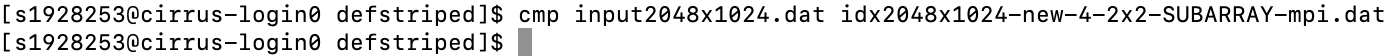
\includegraphics{logos/cmp.png}}
\end{center}
\caption{Write bandwidth for local data volume n = 128}
\label{fig:eucrest}
\end{figure}

\section{Final Proposal}
For this project, there are several things I need to do during the whole period:

\begin{enumerate}
    \item Convert the original code to C version
    \item Check the results(output files) and performance
    \item Run on different HPC systems
    \item Extend it to irregular patterns
    \item Re-run it on different machines
\end{enumerate}
\subsection{Convert to C}
The first work I need to do is converting Jiaying's code to a new C version. There are two reasons. One is there already exists Fortran version, I want to improve this program based on previous work. The other is considering that most HPC classmates and I are C programmer, it would be more familiar and understandable for students.

To complete this task, one crucial thing is to understand the entire contents of the source code, and the primary logic file \textit{benchmark.f90} has 416 lines of code. It is necessary to make clear what methods did she use, what data types and data structures were included. After these, we can begin creating a new version in C using the same idea.

\subsection{Check the results and performance}
If the program has no error, the output file should be the same with the input file. We can use this feature to inspect if the C program is correct. Then we can observe whether the C program has the same performance as the source program. We should compare the amount of time used and the IO read and write rate.

\subsection{Run on differents machines}
We better be able to run the two programs on HPC machines, such as ARCHER, Cirrus. Because we want to know the performance of each program running on different machines and make a comparison as well.
The best case is that we could run the code on as many machines as possible, which means different Makefiles are needed because of different environments among those machines.

However, ARCHER may be unavailable in several weeks. Hence, at least we need to promise they can run on Cirrus successfully. If we can have ARCHER 2 at that time, it is also necessary to test the programs on it.

% To compare the performance of these programs on different machines, we still need to use variable controlling method. Which means running these two programs using various numbers of processes. Then compare how long they spend separately.

\subsection{Extend to an irregular pattern}
A critical function I want to implement in this project is to extend the original method of decomposition to an irregular pattern. Because a benchmark program needs to simulate real-life programs, many of the high performance IO programs cannot have a strictly regular decomposition. Hence, I want to investigate will performance be affected if we let the processes read the data in memory randomly.

All previous work includes benchio, the previous dissertation used regular decomposition, as shown in Figure 5.
 
\begin{figure}[h]
\centering
\begin{minipage}[t]{0.5\textwidth}
\centering
\resizebox{1.00\hsize}{!}{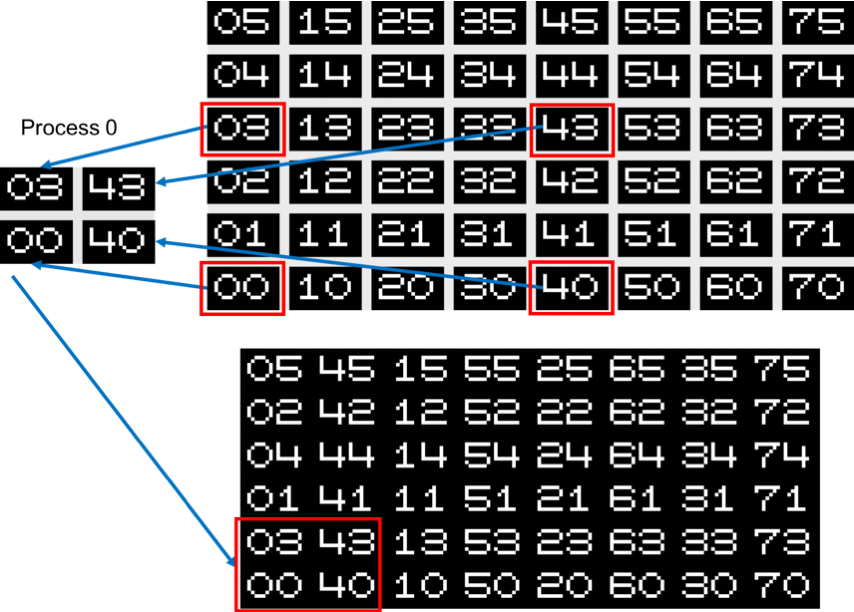
\includegraphics{logos/regular.png}}
\caption{Regular decomposition; extracted from the benchmark paper[1]}
\end{minipage}
\begin{minipage}[t]{0.48\textwidth}
\centering
\resizebox{1.00\hsize}{!}{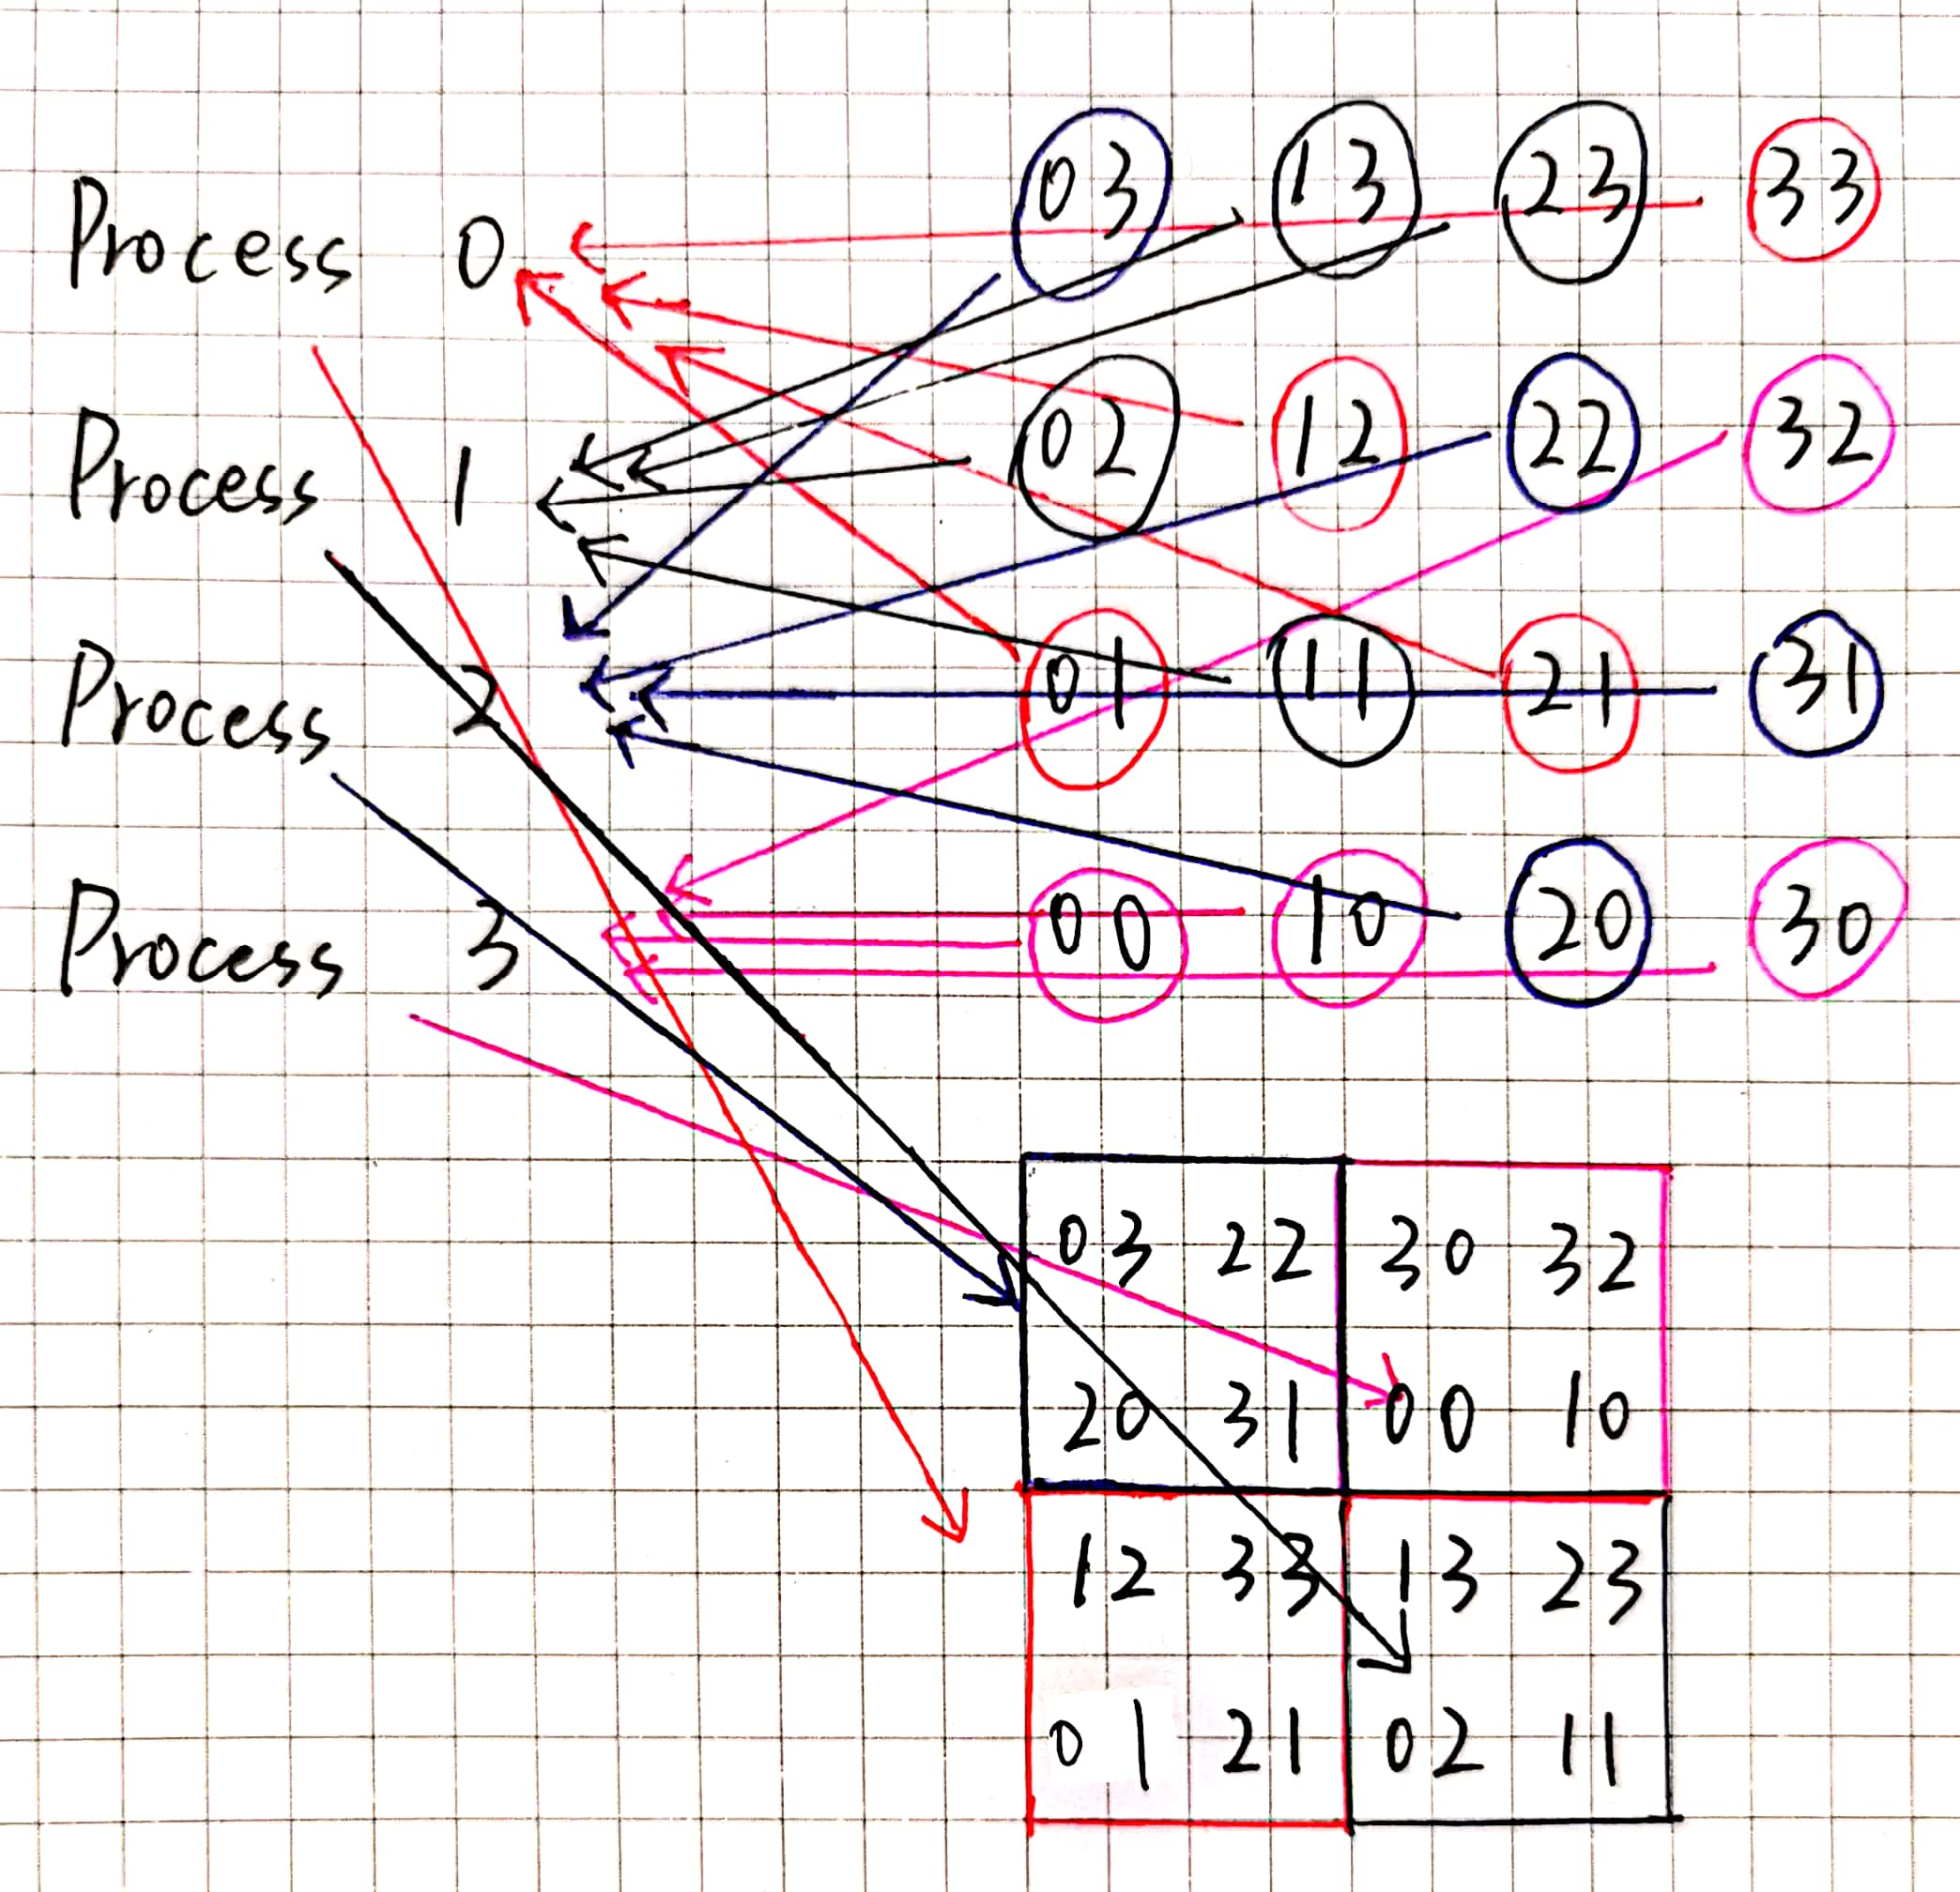
\includegraphics{logos/irregularpattern.jpeg}}
\caption{Irregular decomposition}
\end{minipage}
\end{figure}

From the figure, we can see that process 0 reads block-cyclic distributed arrays stored in the test image, then writes in a block mapping to a common output.

What we want to implement in this project is that let processes read the array randomly, as shown in Figure 6.

There is a four-process example from number 0 to 3. Each process randomly reads four blocks of data in the local data set, and we can locate where the data comes from based on the picture content. Then write the data to the common output.
When we do a regular pattern, we open the file, write the file, we have to tell the process which data from which part of memory.
We also need to create a random number generator to do it randomly.

This irregular approach may increase the complexity of the problem. However, this situation is closer to the real application. We need to use this benchmark to simulate this situation.

\pagebreak

\section{Workplan}
This is the Gantt chart of the entire project:

\begin{figure}[h]
\begin{center}
\resizebox{0.99\hsize}{!}{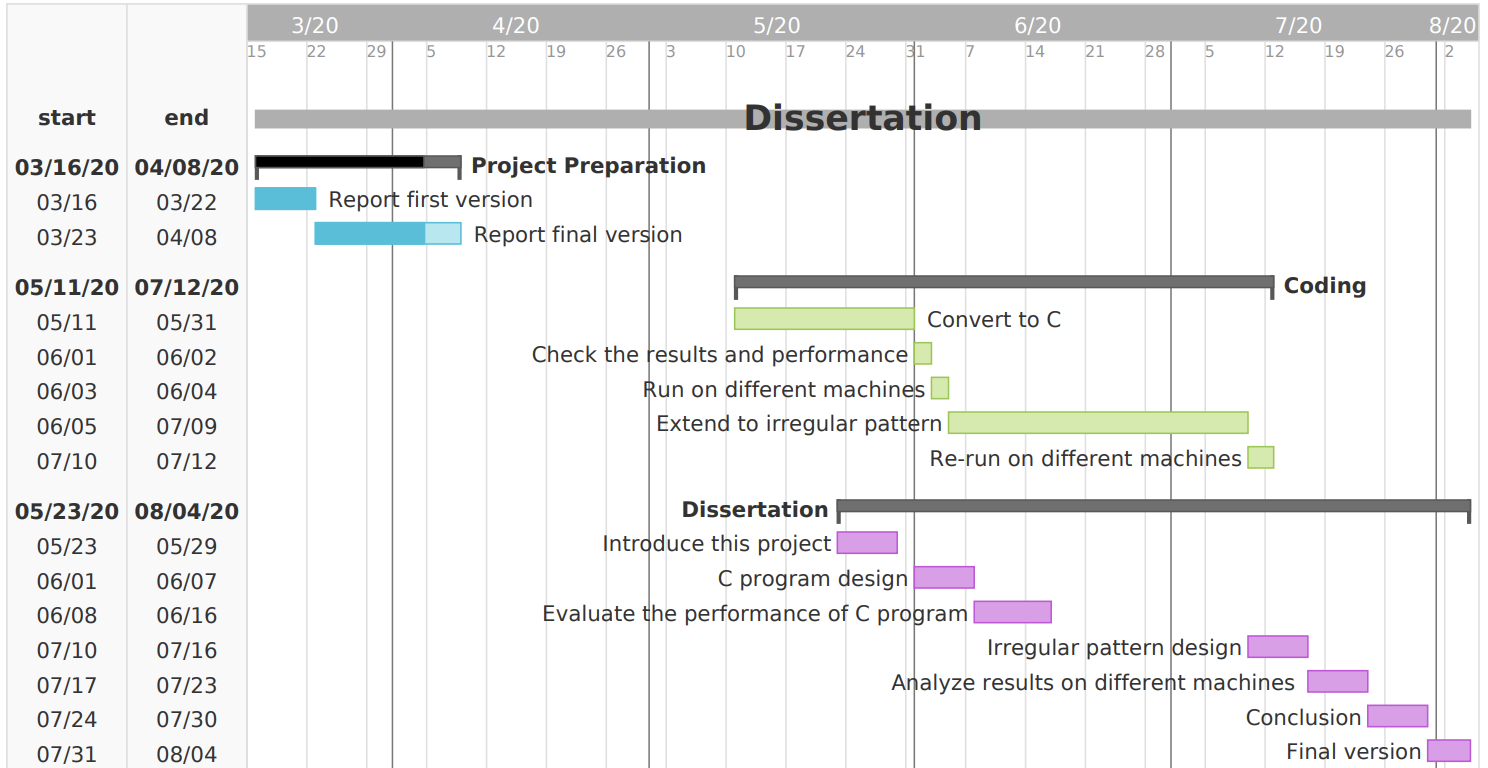
\includegraphics{logos/gantt.png}}
\end{center}
\caption{Gantt Chart for Workplan}
\label{fig:eucrest}
\end{figure}

\section{Risk Analysis}
This part will discuss what could go wrong during the whole project and issues which are probably encountered.

\subsection{Converting code to C}
Converting a Fortran program into a C program requires us to be clear about the function of each line of code. This is the first job for the whole project. If it cannot be completed, the next work will be difficult. The probability of this risk occurring is very tiny, I think based on my C language foundation and David's help, I will complete this task successfully.

To make the program proceed, we can use the programs written before, such as coursework of MPP courses. We can use this program as a basis, improve this program, and finally achieve the desired functions.
\subsection{Whether I can access to the machines in the future}
We want to run the program on as many machines as possible. However, because ARCHER may be unavailable in a few weeks. I am not sure what machines I can use at that time.

However, at least I need to make sure I can access Cirrus, although ARCHER 2 will probably not be available soon.
\subsection{Irregular pattern}
This scheme is not included in the previous work, and it is a challenge for how to design irregular decomposition and how to write them to common output.

In order to complete this work, I need to study multiple decomposition methods, look for the similarities and differences between them to create an irregular pattern.
\subsection{What would happen if I return to China}
Due to the severe situation of Covid-19. The university has informed students to return to their hometown if it is possible. I plan to return to China by air on 28 May 2020. This is very likely to happen and the most critical risk because China has now controlled the epidemic. I am not sure if I can continue to use the machines in the university because of the long-distance after returning to China. Another issue is I can only have online meetings with my supervisor. we now use Microsoft Teams, I do not know how efficient this is and whether we can solve all the problems online.

These situations may happen. Hence I will install open-mpi, Fortran and C compilers on my laptop. Although it cannot test IO performance, at least I can test whether the program works. If Microsoft Teams cannot be used in China, I will consider using VPN or contact by email.

\subsection{Hard to get reliable performance on any machine}
When we take IO operations, the time consumed will vary a lot. Because IO operations are relatively time-consuming. We need to run the programs lots of times to obtain a constant value. There is also a high probability that this risk will occur.

\subsection{Other IO libraries}
If time permits, I would like to look at other IO libraries such as NetCDF, HDF5, make comparisons with MPI-IO. However, this is a new attempt, whether Cirrus and ARCHER support other libraries is uncertain. Probably the functions will be limited.

Whether we can use other libraries, make sure MPI-IO works normally is the first task. If we have time, investigate other libraries' performance would also be considered. This risk may not be very urgent because the primary library in this project is MPI-IO. 

\section{Outline of the Dissertation Report}

\begin{enumerate}
	\item Introduction
	\item Background theory
	\begin{enumerate}
		\item benchio
		\item previous dissertation
		\item Parallel IO Libraries
		\item Lustre File System
	\end{enumerate}
	\item Experimental design
	\begin{enumerate}
		\item Code Design
		\item Testing Design
	\end{enumerate}
	\item Results
	\item Analysis
	\item Conclusion
\end{enumerate}

\pagebreak
\begin{thebibliography}{100}

\bibitem{ref:Wu} J.Wu. {\em 2016 Parallel IO Benchmarking.} Online at  \url{https://static.epcc.ed.ac.uk/dissertations/hpc-msc/2015-2016/Jia-ying_Wu-MSc-dissertation-Parallel_IO_Benchmarking.pdf}

\bibitem{ref:benchio} D.Henty, A.Jackson, C.Moulinec, V.Szeremi. {\em 2015 Performance of Parallel IO on ARCHER.} Online at \url{http://www.ARCHER.ac.uk/documentation/white-papers/parallelIO/ARCHER_wp_parallelIO.pdf}

\bibitem{ref:archer} {\em Parallel I/O Performance Benchmarking and Investigation on Multiple HPC Architectures.} Online at \url{http://www.ARCHER.ac.uk/documentation/white-papers/parallelIO-benchmarking/ARCHER-Parallel-IO-1.4.pdf}

\end{thebibliography}


\end{document}